\documentclass[draft]{article}
\usepackage[utf8]{inputenc}
\usepackage[spanish]{babel}
\usepackage{graphicx}	%Si se quiere compilar con las imagenes
% \usepackage[draft]{graphicx}	%Si NO se quiere compilar con las imagenes porque tarda mucho
\usepackage{graphics, float, fancyhdr, titling, caption, subcaption}
\usepackage{listings}
\usepackage[a4paper, total={6in, 9.5in}]{geometry}
\usepackage{fancyhdr}
\usepackage{hyperref}		% solo se debe usar si se quiere usar \hypersetup
\usepackage{xurl}


% \usepackage{amsmath}      % Si se quiere usar \text{texto} dentro del modo matematico
%\setcounter{secnumdepth}{-2}       %Poner solo esto si no se quieren numero delante de las secciones y niveles inferiores.

\renewcommand{\footrulewidth}{0.4pt}
\title{

\includegraphics[width=1.75in]{imagenes/UGR-Logo.png} \\
\vspace*{1in}
\textbf{Cuestiones Tema 4} \\
Animación por Ordenador \\
\vspace*{0.5in}}
\author{Andrés Merlo Trujillo \\
andresmerlo@correo.ugr.es \\
77147239H \\ 
\vspace*{0.5in} \\
E.T.S. de Ingenierías Informática y de Telecomunicación \\
\textbf{Universidad de Granada}} \date{\today}

\hypersetup{
    colorlinks=true,
    linkcolor=black,
    citecolor=black
}

\renewcommand\maketitlehooka{\null\mbox{}\vfill}
\renewcommand\maketitlehookd{\vfill\null}

\begin{document}
\begin{titlingpage}
\maketitle
\end{titlingpage}

\tableofcontents

\newpage

\pagestyle{fancy}   %a partir de comienza el header (se salta el indice y portada)
\fancyhead[L]{Andrés Merlo Trujillo}
\fancyhead[R]{Animación por Ordenador}
%\section{Ejercicio 1}
%\begin{figure}[H]
%    \centering
%    \includegraphics[width=\textwidth]{imagenes/passwdfile.png}
%    \vspace{10pt}
%    \footnotesize{Fuente: https://...}
%\end{figure}

% \begin{figure}[H]\ContinuedFloat		% si se parten las imagenes en dos paginas y se desea continuar las letras de las subfiguras (a, b, c, ..., otra pag -> c, d, e)
% \begin{figure}[H]
%     \centering 
% 	\begin{subfigure}[t]{0.48\textwidth}
% 	    \centering
% 	    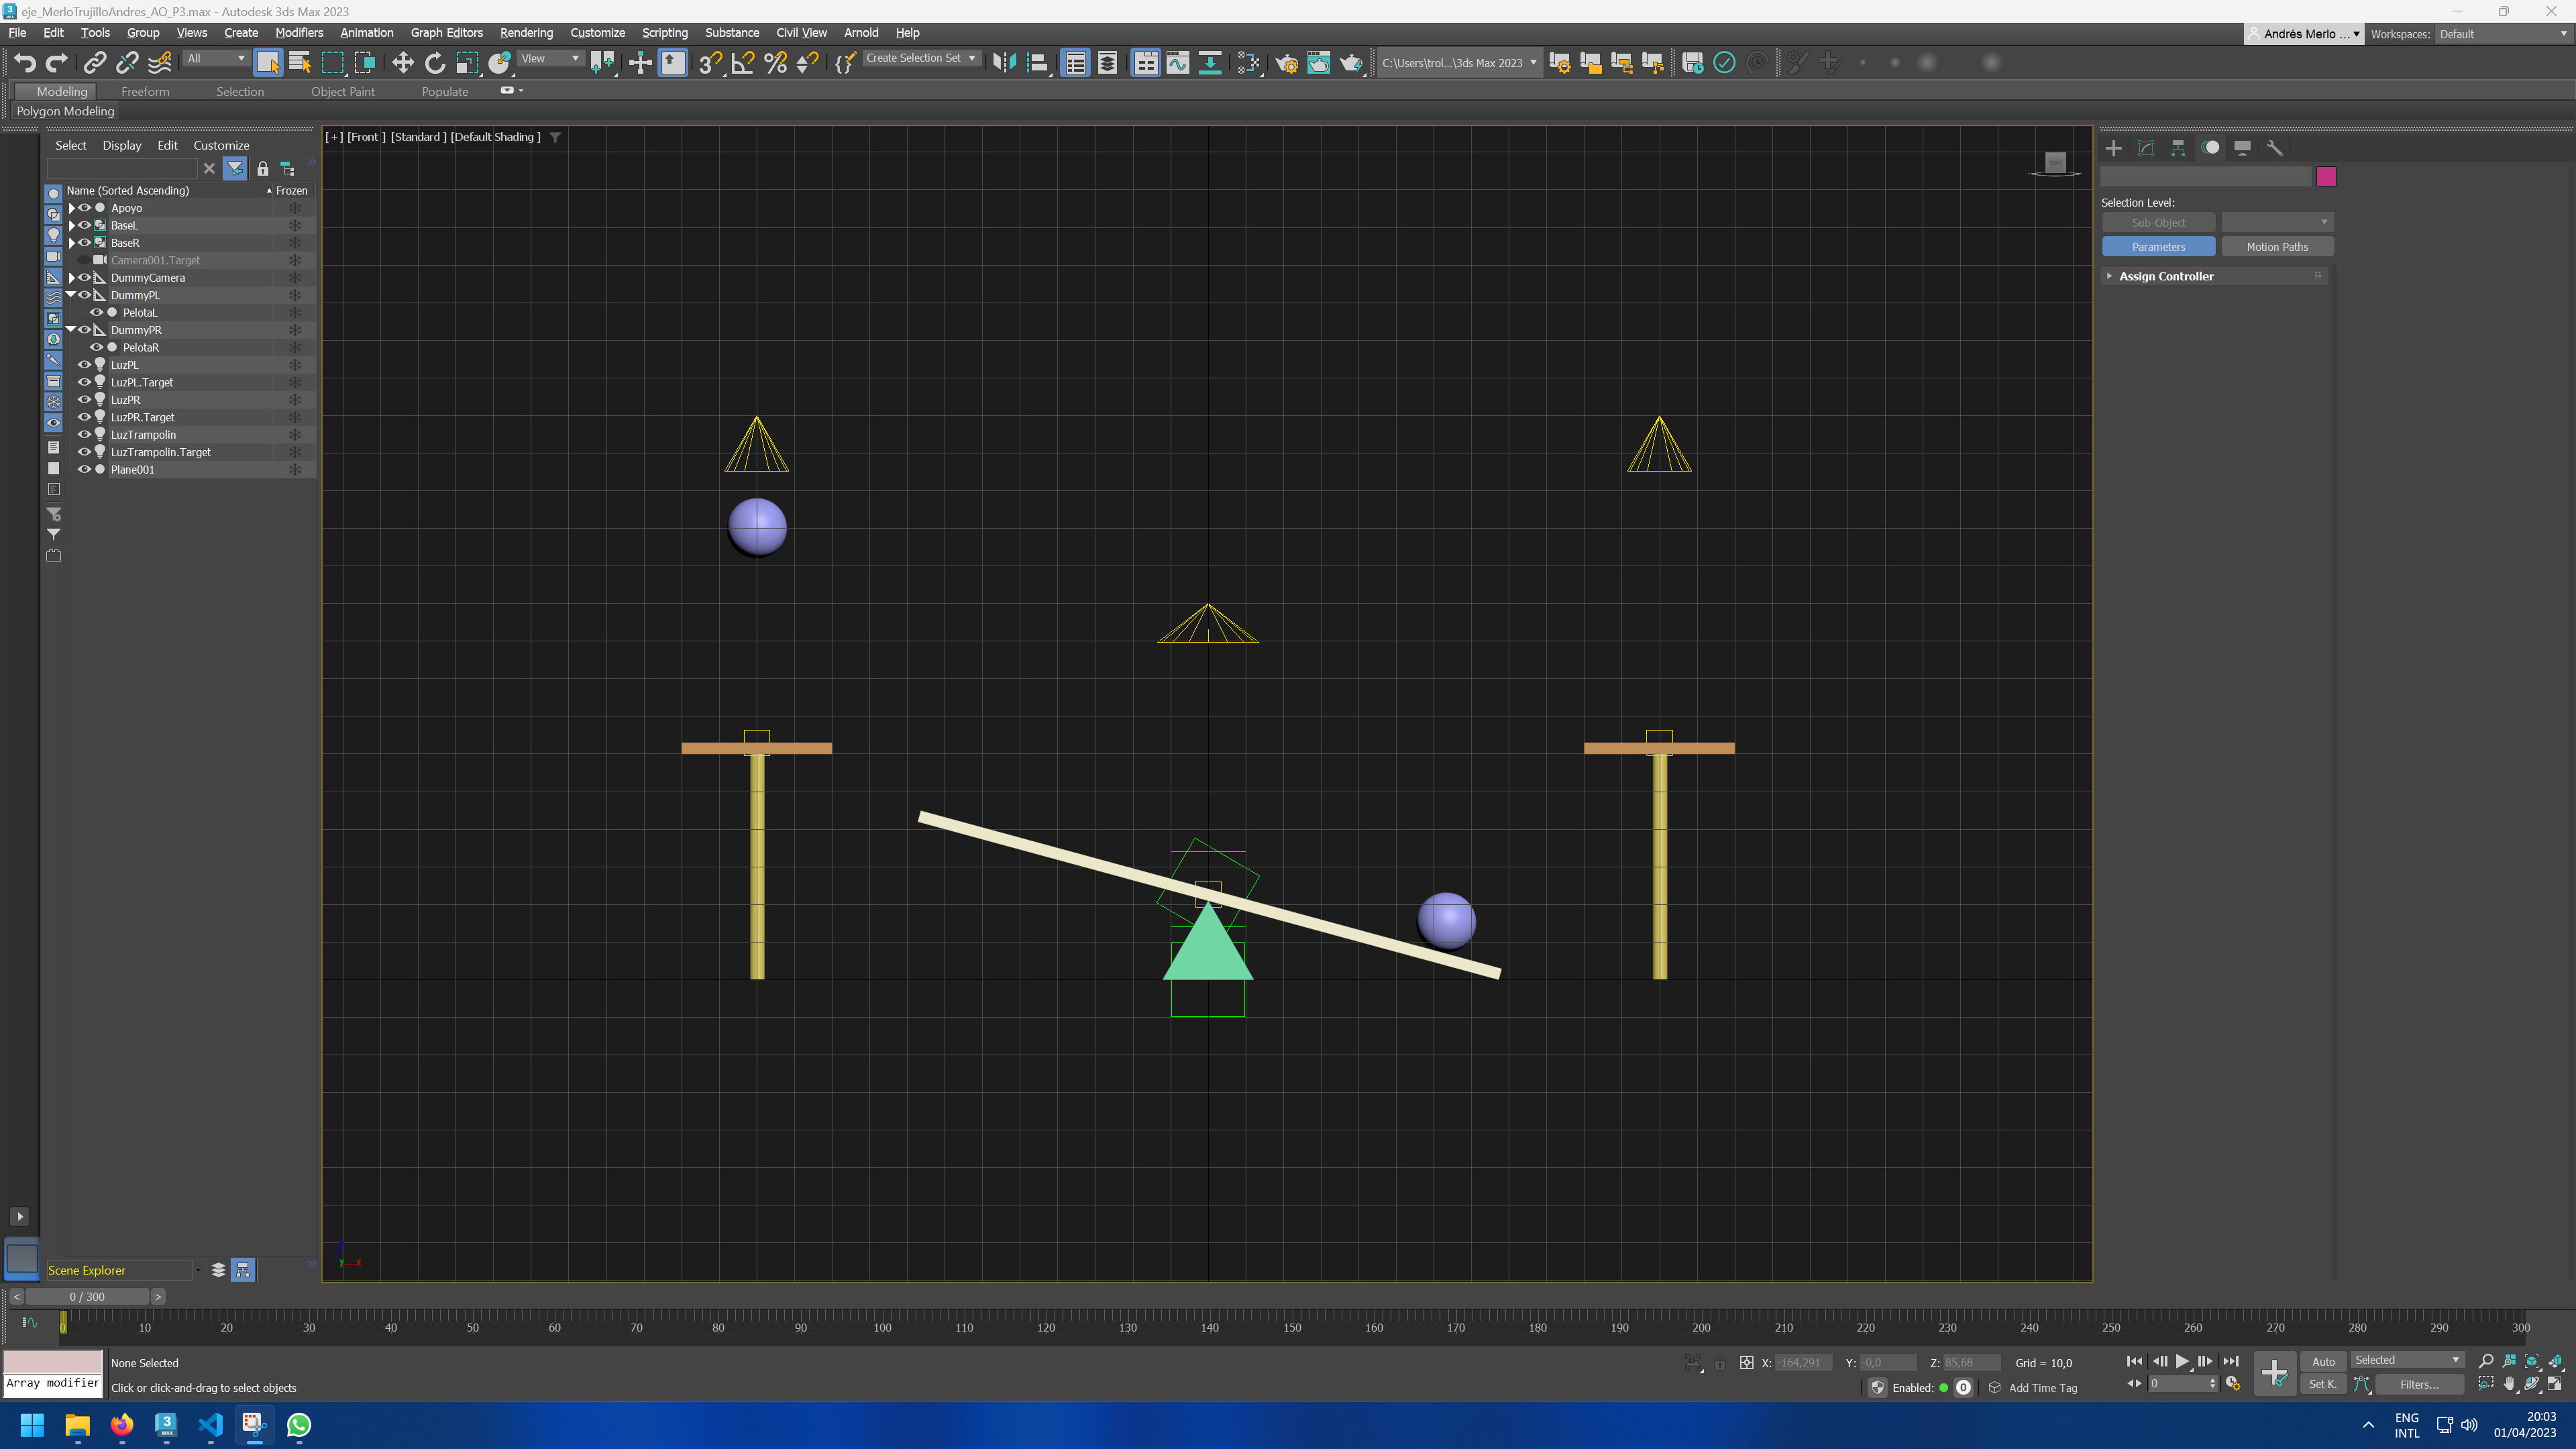
\includegraphics[width=\textwidth]{imagenes/Ejercicio 1/keyframes/0.png}
%         \caption{Pelotas en el instante 0.}
%     \end{subfigure}
%     \hfill
%     %\par\bigskip %si se desea dejar un margen entre la imagen de arriba y de abajo
% 	\begin{subfigure}[t]{0.48\textwidth}
% 	    \centering
% 	    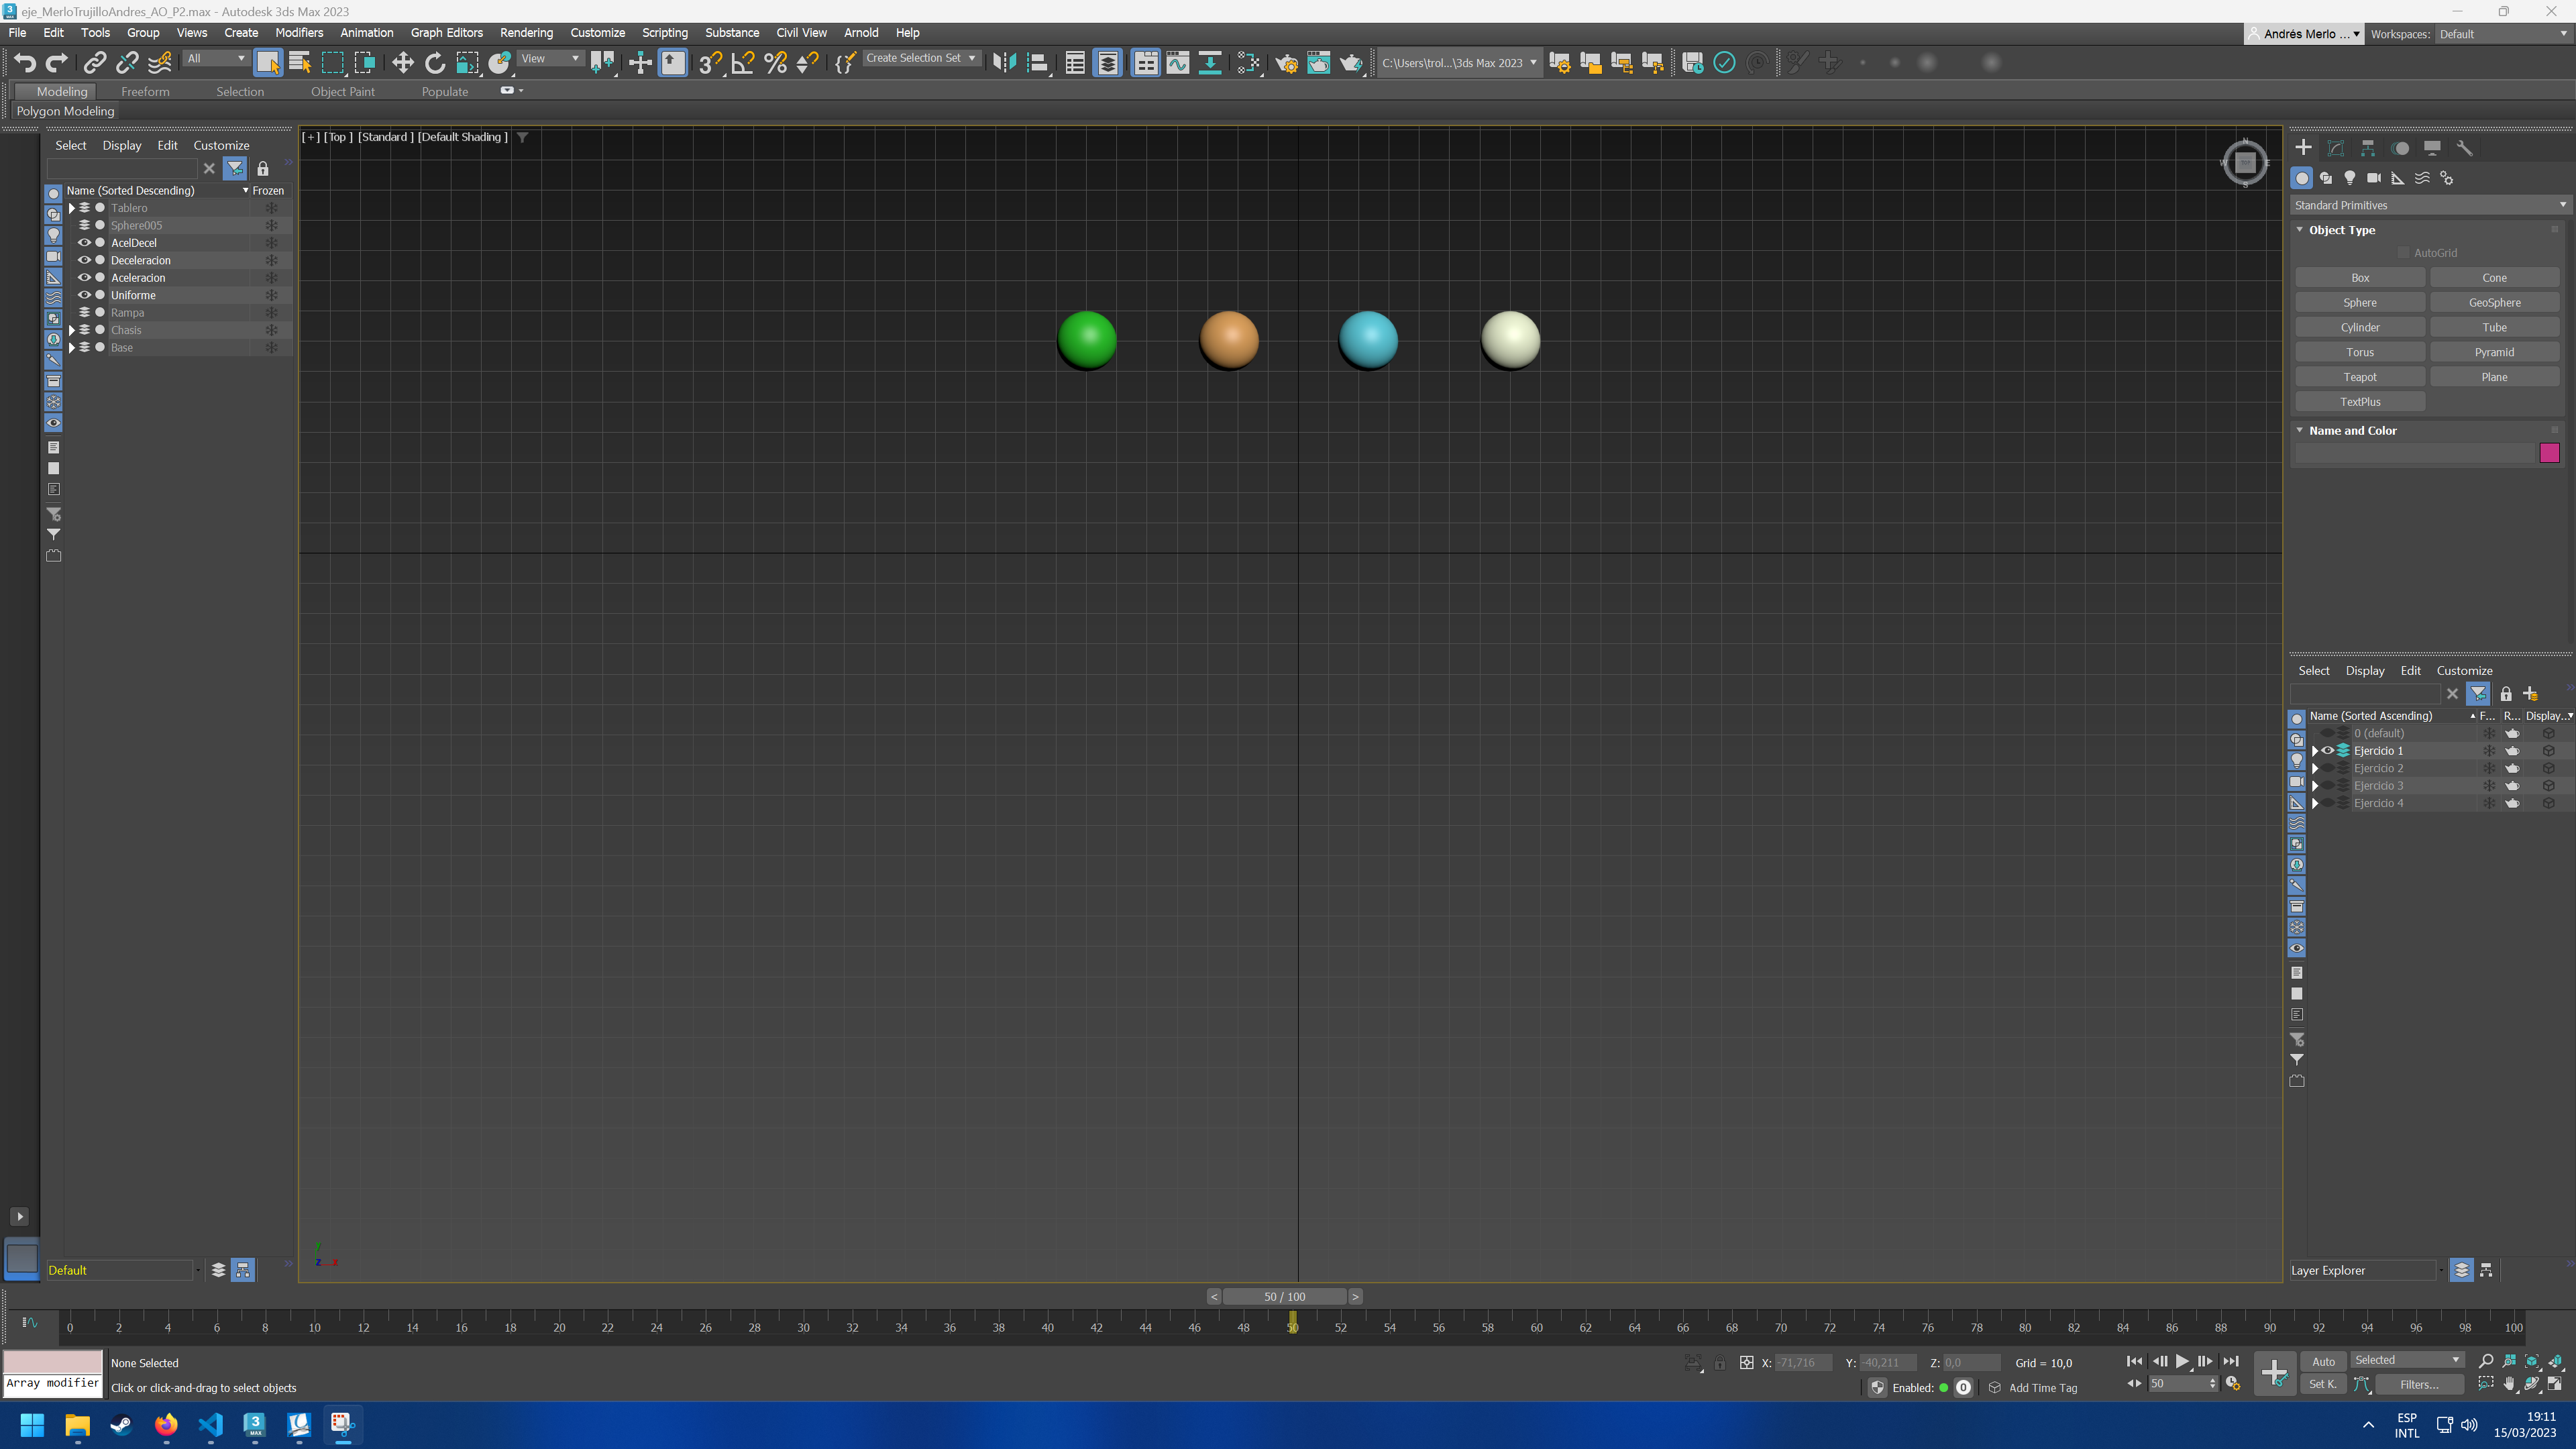
\includegraphics[width=\textwidth]{imagenes/Ejercicio 1/keyframes/50.png}
%         \caption{Pelotas en el instante 50.}
%     \end{subfigure}    
% \end{figure}

% $30 \text{fps} \times 2 \times 5 \text{segundos} = 300 \text{fotogramas} $

\section{Localiza en 3DS Max estos canales e indica qué serían cada uno de ellos.}

Los canales en 3DS Max se pueden ver en el editor de curvas, con un objeto seleccionado. Además, estos canales dependen de la animación que se haya hecho para dicho objeto, por lo que puede ser variable. 

% foto de un cubo
\begin{figure}[H]
    \centering
    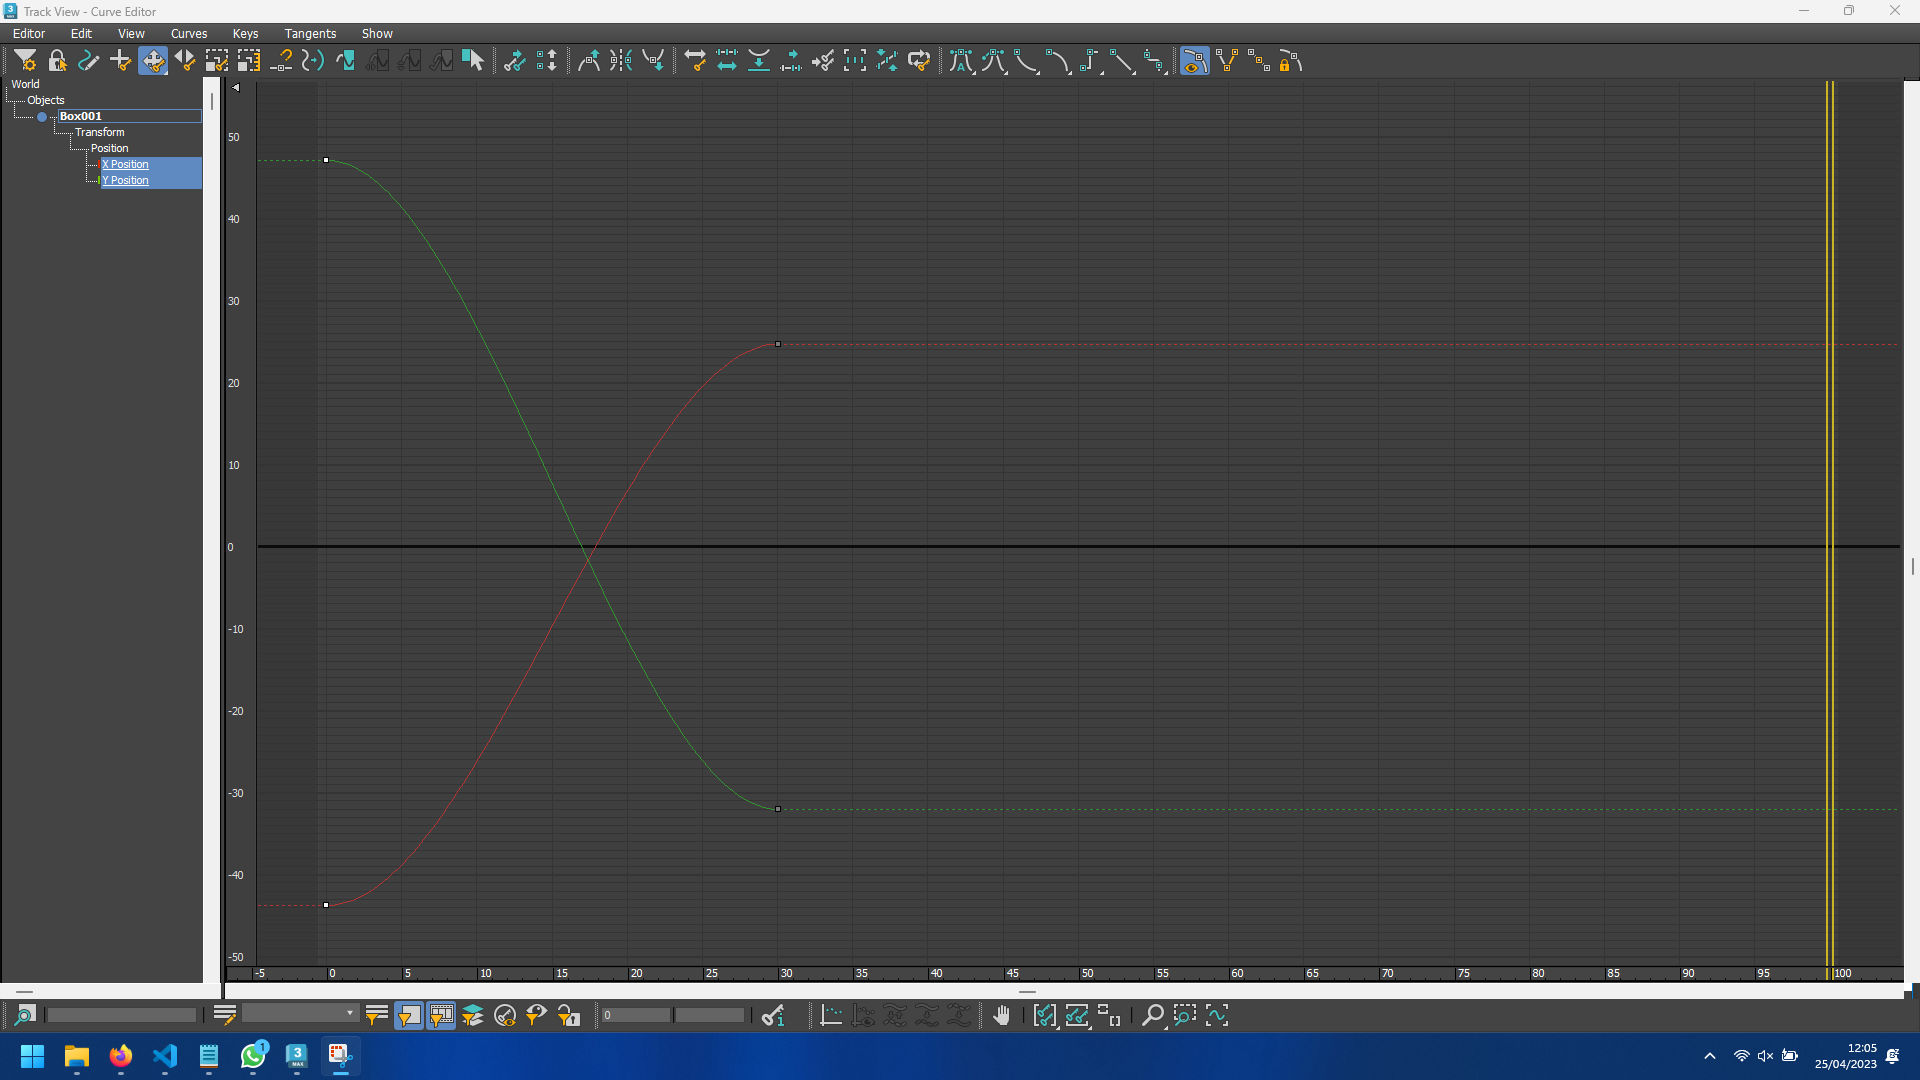
\includegraphics[width=\textwidth]{imagenes/11.png}
    \caption{Canales del cubo.}
\end{figure}

En el caso del cubo, se puede ver que tiene dos canales: el de posición en el eje X y el de posición en el eje Y.

\begin{figure}[H]
    \centering
    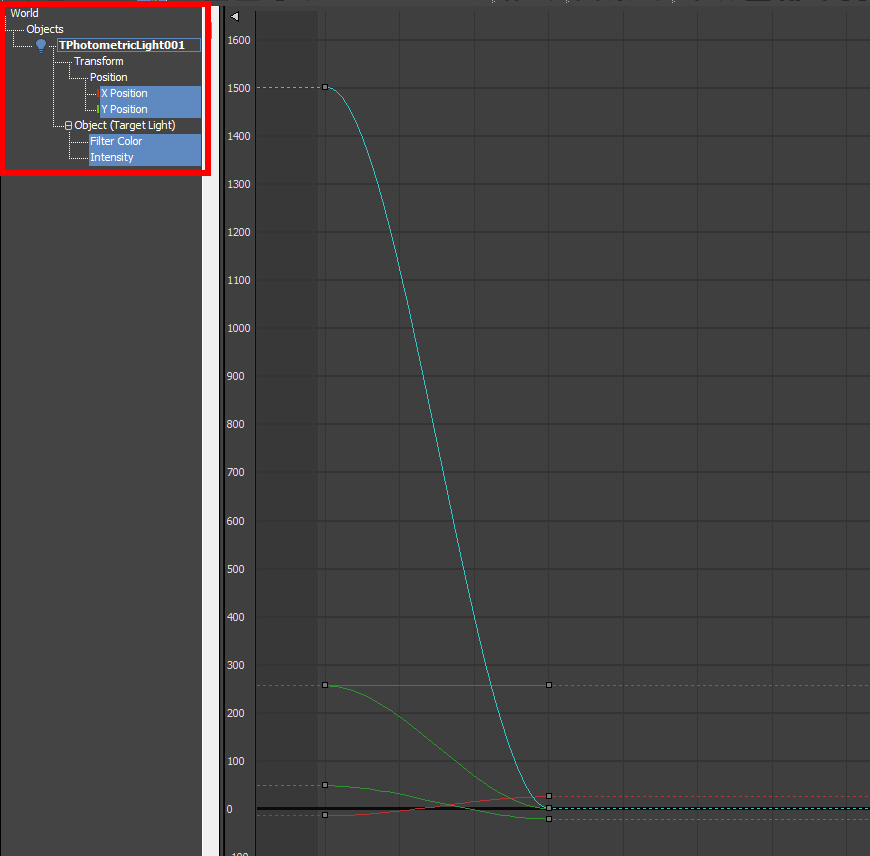
\includegraphics[width=\textwidth]{imagenes/12.png}
    \caption{Canales del \textit{Target Light}.}
\end{figure}

En este caso, la luz tiene 4 canales: los mismos que el cubo para la posición en el eje X e Y, el color de la luz y su intensidad.

\bigskip

Por tanto, se puede decir que el número de canales viene determinado por cada ``curva'' que tenga el objeto asociado; es decir, por el número de atributos que se anime en el objeto.


% mejorar
\section{Indica las ventajas e inconvenientes trabajando con poses frente a canales.}

Ventajas de trabajar con poses: 

\begin{itemize}
    \item Más rápido a la hora de reproducir animaciones, ya que el vector indica directamente las propiedades del objeto en un momento dado.
    \item Almacenamiento contiguo en memoria, lo que permite un acceso más rápido por parte del procesador.
\end{itemize}

\bigskip

Desventajas de utilizar poses:

\begin{itemize}
    \item Dificultad para añadir o eliminar canales, al ser necesario modificar la estructura del vector en todos los instantes.
\end{itemize}

Ventajas de trabajar con canales:

\begin{itemize}
    \item Posibilidad de optimizar el almacenamiento de la estructura de datos, al ser independientes una de otras.
    \item Independencia entre canales, permitiendo añadir o eliminar nuevos canales de forma rápida y directa.
\end{itemize}

Desventajas de utilizar canales:

\begin{itemize}
    \item Necesidad de evaluar de forma independiente cada canal para saber que atributos tiene la escena en un momento dado. Esto implica acceso a cada canal, que no está en memoria de forma contigua, haciendo que se requiera tiempo y cómputo adicional.
\end{itemize}

\section{¿Qué tipo de interpolación hace por defecto 3DS Max entre dos fotogramas clave definidos manualmente en términos de \textit{spacing}?}

Para saber que tipo de \textit{spacing} se utiliza, es necesario animar un objeto para que se mueva de un lado a otro y después ver su \textit{Motion Path}.

% Foto de la animacion
\begin{figure}[H]
    \centering
    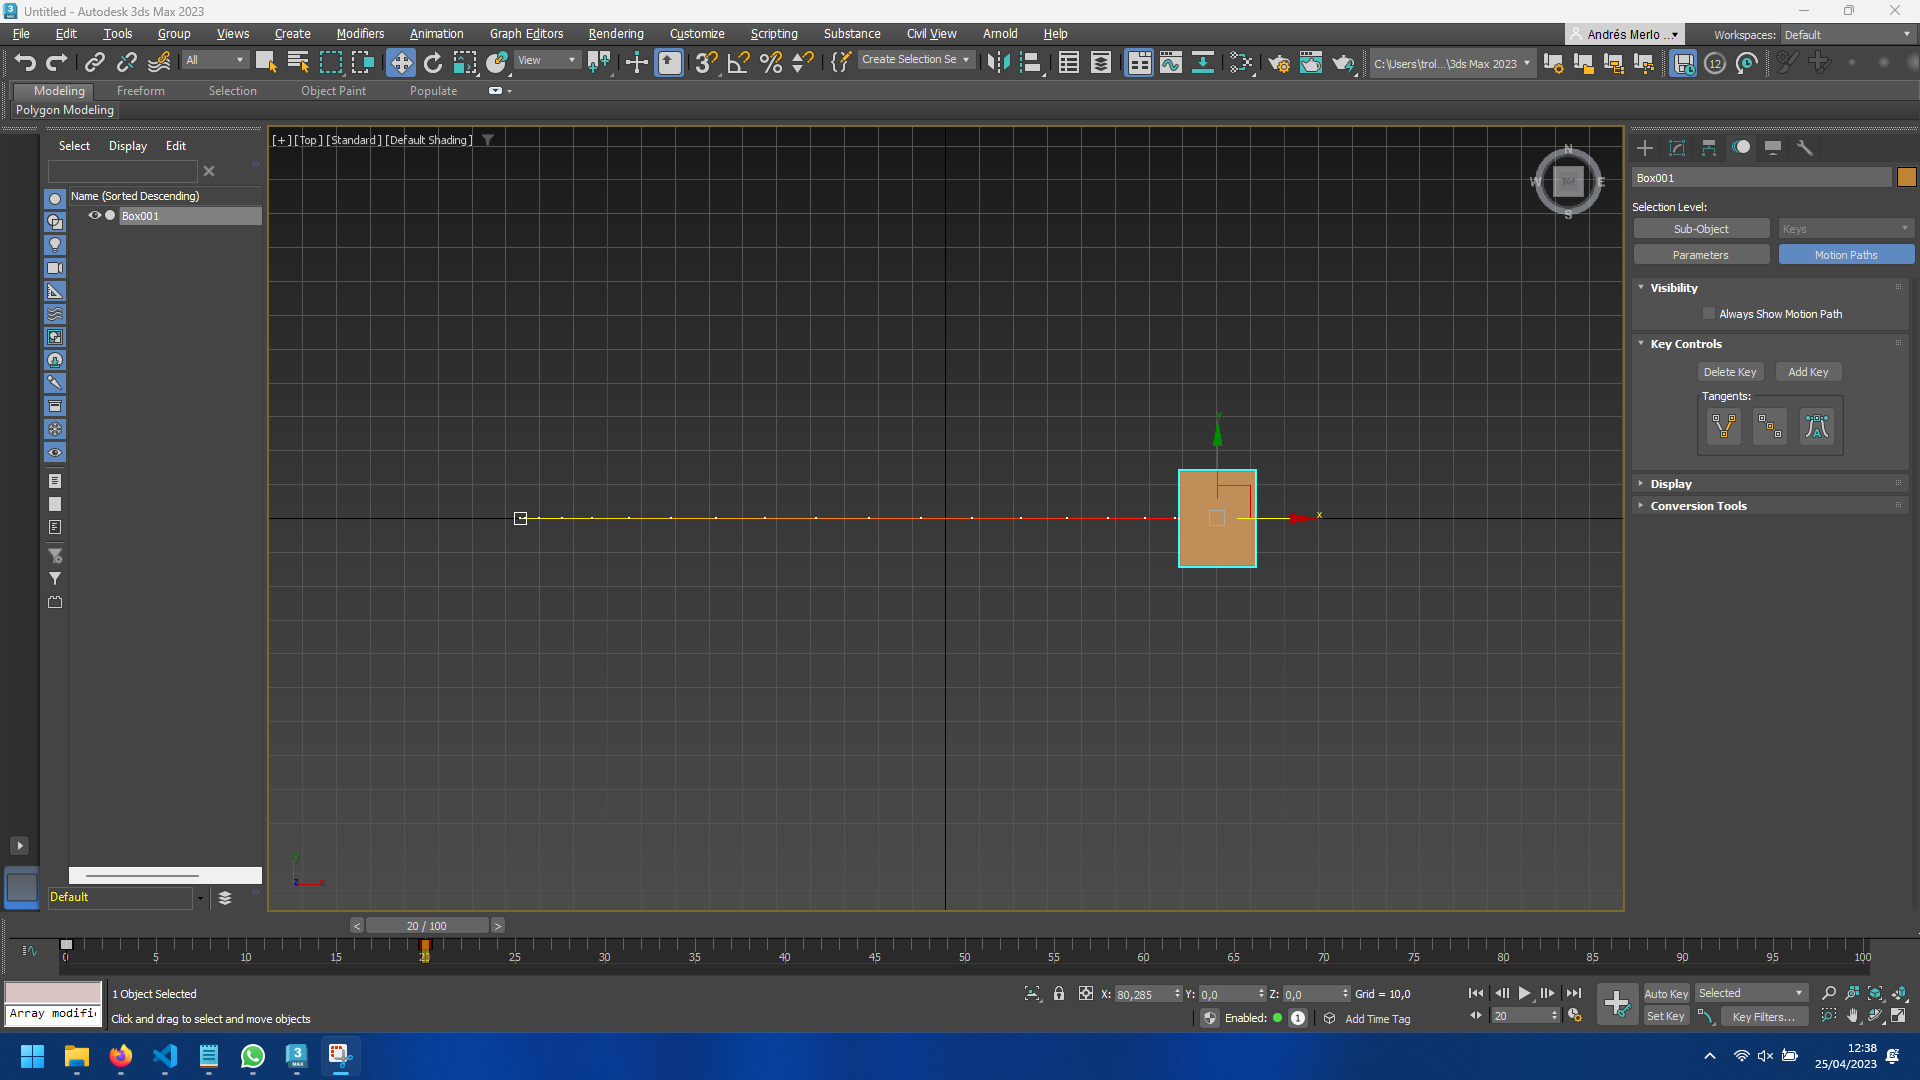
\includegraphics[width=\textwidth]{imagenes/3-1.png}
    \caption{\textit{Motion Path} seguido por un cubo animado.}
\end{figure}

% Como se puede ver, el número de puntos es mayor y más cercanos en los bordes que en el centro, dando a entender de que se sigue un espaciado no lineal.
Como se puede ver, sigue una línea recta, dando a entender que sigue una interpolación línea. No obstante, también se puede ver que el número de puntos es mayor en los bordes y menor en el centro, por lo que es no uniforme. 


% escribir sobre mas puntos
\section{¿Qué información almacena un fotograma clave?}

Para ver que información almacena un fotograma clave en 3DS Max, es necesario animar un objeto e irse al editor de curvas. A continuación, es necesario seleccionar un punto de cualquier curva y darle clic derecho.

\bigskip

Aparecerá la siguiente ventana:

% foto de la ventana
\begin{figure}[H]
    \centering
    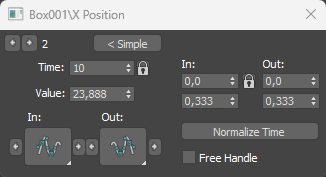
\includegraphics[width=\textwidth]{imagenes/4-1.png}
    \caption{Ventana con los datos que almacena para cada fotograma clave.}
\end{figure}

A la izquierda se puede ver que almacena el valor del atributo y el instante en el que se produce. A la derecha se puede ver que almacena dos pares de valores, que modifican los puntos de control de ese fotograma clave.

\begin{figure}[H]
    \centering
    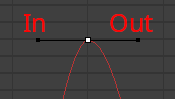
\includegraphics[width=\textwidth]{imagenes/4-2.png}
    \caption{Puntos de control del fotograma clave.}
\end{figure}

De estos pares de valores, el de arriba modifica la posición en el eje Y (vertical) del punto de control y el de abajo modifica la longitud desde el fotograma clave hasta el punto de control.

\section{¿Por qué puede ser tan importante considerar el sistema de referencia en una animación?}

\subsection{Da un ejemplo en el que la animación varíe dependiendo del sistema de referencia.}
\section{Ejercicio 6}
\section{Ejercicio 7}

\end{document}
